\section{Topology}

\begin{definition}
  Let $X$ be a set and $\mc T$ a collection of subsets of $X$.

  $\mc T$ is a \defn{topology} and $(X, \mc T)$ is a \defn{topological space} if
  \begin{enumerate}
  \item $\emptyset \in \mc T$ and $X \in \mc T$
  \item $\mc T$ is closed under arbitrary (including uncountable) unions
  \item $\mc T$ is closed under finite intersections.

  An \defn{open set} is an element of $\mc T$.
\end{enumerate}
\end{definition}


Let $(X, d)$ be a metric space. We define a set $G$ to be an \defn{open set in the metric space sense} if for
every $x \in G$ there exists $r > 0$ such that $B(x, r) \subseteq G$.

The topology generated by $d$ is the collection of all sets that are a neighborhood of all their points:
  \begin{align*}
    \mc T = \{ G \subseteq X ~:~ \forall x \in G ~ \exists \eps ~ B(x, \eps) \subseteq G \}
  \end{align*}
\begin{lemma}
  The collection of open sets in the metric space sense is a topology.

  We call this the \defn{topology generated by the metric} $d$.
\end{lemma}

OK, so the topology induced by the metric is the collection of all sets that are open according to the metric.
So consider the points $1$, $2$, and $3$ in $\R$. You might think that the induced topology tells us that $3$
lies in between the other two? Perhaps because we never see an open set that contains $1$ and $3$ but not $2$?
But no, that doesn't work : e.g. $(0, 1.5) \cup (2.5, 3.5)$. In fact it's not true that the topology tells use
the ordering of those 3 points. Ordering isn't a topological property; this is something to do with the order
relation on $\R$.

\url{https://mathoverflow.net/questions/19152/why-is-a-topology-made-up-of-open-sets}


\begin{proof}
  Let $\mc T$ be the set of open sets in the metric space sense.

  Let $U, V \in \mc T$.

  First, we must show $U \cap V \in \mc T$. Let $x \in U \cap V$. Then there exists $B(x, r_U) \subseteq U$
  and $B(x, r_V) \subseteq V$. Therefore $B(x, \min(r_U, r_V)) \subseteq U \cap V$. Hence $U \cap V$ is open
  in the metric space sense and therefore $U \cap V \in \mc T$.

  Finally we must show an arbitrary union $\bigcup \mc U \in \mc T$. Let $x \in \bigcup \mc U$. Pick any open
  set containing $x$ and use a ball from that open set. That ball is in $\bigcup \mc U$.
\end{proof}

\begin{lemma}
  \begin{enumerate}
  \item Every open ball is open in the metric space sense.\\
    (This doesn't seem to have anything to do with topology, we're just proving that the ``open
    ball​'' is open in the metric space sense)\\
    ({\bf proof}: basically given $y \in B(x, \eps)$ take $B(y, \eps - d(x, y))$)

    Given $y \in B(x, \eps)$ we must exhibit $\delta$ such that $B(y, \delta) \subseteq B(x, \eps)$,
    i.e. such that $d(x, z) < \eps$ for all $z \in B(y, \delta)$.

    By the triangle inequality we have $d(x, z) \leq d(x, y) + d(y, z)$. Thus we
    want $d(x, y) + d(y, z) < \eps$, which we can achieve by setting $\delta = \eps - d(x, y)$.


  \item Every open set can be written as a union of open balls.\\

    This is immediate. By definition every point in an open set (metric sense) has a ball around
    it. Take the union of those balls.
  \end{enumerate}
\end{lemma}




The \defn{discrete topology} consists of {\it all subsets} of $X$.

The \defn{trivial topology} (or ``\defn{indiscrete topology}​'') consists of $\emptyset$ and $X$.


\url{https://www.youtube.com/watch?v=UQas4Cu89D0}

\begin{remark*}
  \url{https://math.stackexchange.com/a/2614297/397805}

  Every function on the discrete topology is continuous.

  {\bf Proof}: every subset is open, therefore every preimage is open.

  Every continuous function on the indiscrete topology is constant.

  {\bf Proof:} Let $f$ be continuous on the indiscrete topology. Then every preimage is $X$. Consider $x_1$ and
  $x_2$ in the domain. Pick any open set in the codomain: it contains both $f(x_1)$ and $f(x_2)$....
  Let $x_1, x_2 \in X$. Let $G_1$ be an open set containing $f(x_1)$. Then $f^{-1}(G_1)$ must be $X$ (since it
  cannot be $\emptyset$). Therefore $f(x_2) \in G_1$. So
  \red{TODO}
  \url{https://math.stackexchange.com/a/1770507/397805}
\end{remark*}



\begin{definition}
  \defn{interior point}

  \defn{interior}

  \defn{limit point}

  \defn{accumulation point}

  \defn{closure}

  \defn{boundary}

  \defn{isolated point}

  \defn{neighborhood}
\end{definition}

\begin{theorem}
  A countable union of closed sets is closed.

  An uncountable intersection of closed sets is closed.
\end{theorem}

\begin{proof}
  $\bigcup_i F_i = \(\bigcap F_i^c\)^c$, which is the complement of a finite intersection of open sets (open),
  and therefore closed .

  $\bigcap_{F \in \mc F} F = \(\bigcup_{F \in \mc F} F^c\)^c$ which is the complement of an arbitrary
  intersection of open sets (open), and therefore closed.
\end{proof}

\begin{theorem}
  If $A \subset X$ then
  \begin{align*}
    \bar A = \bigcap \{\bar F ~:~ F \text{~closed}, F \supset A\}
  \end{align*}
  and $\bar A$ is closed.
\end{theorem}

\begin{proof}
  \red{TODO}
\end{proof}

\begin{definition}[basis]
  A collection of open sets $\mc B$ is a \defn{basis} for a topological space if for every $x, U$ with
  $U$ open and $x \in U$ there exists $B \in \mc B$ such that $x \in B \subseteq U$.
\end{definition}

IOW: a basis is a collection of open neighborhoods​ that are ``everywhere​''. I think they will have to be arranged
in a ``nested​ hierarchy​''. I think that, given a particular basis, if a member $B$ can be written as the union of
other members, then $B$ could be ``pruned​'' from the basis. For $\R$, all intervals is a basis. But any given
interval can be removed from that basis, since the basis contains subintervals that partition it.


\begin{lemma}
  $\mc B$ is a basis iff every $U \in \mc T$ is a union of some subset of $\mc B$.
\end{lemma}

\begin{remark}
  This means that there can only be one topology for a given basis, because we can construct the
  topology from the basis. I think this is because: every element of the basis is in the topology,
  and so the topology must comprise all sets we can make using arbitrary unions.
\end{remark}

\begin{proof}
  $\implies$\\
  Let $\mc B = \{B_\alpha ~:~ \alpha \in I\}$ be a basis and let $U \in \mc T$. We must show that
  there exists $\{B_\alpha ~:~ \alpha \in I\} \subset \mc B$ such that $U = \bigcup_I B_\alpha$.

  Since $\mc B$ is a basis, for each $x \in U$ there exists a subset in $\mc B$ that contains $x$
  and is included in $U$. The union of those subsets equals $U$.

  $\impliedby$\\
  Let $\mc B$ be a collection of subsets and suppose for every $U \in \mc T$ we
  have $U = \bigcup_{\alpha \in I} B_\alpha$ for some index set $I$. We must show that $\mc B$ is a
  basis.

  Let $x \in X$ and $U \in \mc T$. Then $U = \bigcup_{\alpha \in I} B_\alpha$
  and $x \in B_\alpha \subseteq U$ for some $\alpha \in I$.
\end{proof}

We know that a map $f: X \to Y$ is continuous if the preimage of every open set is open. But every
open set is a union of subsets in the basis, and preimage commutes with union, so we expect the
union of preimages of basis subsets to be open.

\begin{lemma}
  Let $\mc B$ be a basis for $\mc T_Y$. A map $f: X \to Y$ is continuous
  iff $f^{-1}(B) \in \mc T_X$ for every $B \in \mc B$.
\end{lemma}

\begin{proof}
  $\implies$\\
  Suppose $f: X \to Y$ be continuous and let $B \in \mc B$. We must show $f^{-1}(B) \in \mc T_X$.
  But $B$ is open so this is immediate.

  $\impliedby$\\
  Suppose  $f^{-1}(B) \in \mc T_X$ for every $B \in \mc B$. We must show $f$ is continuous.

  Let $V \in \mc T_Y$. Then $V = \bigcup_{\alpha \in I} B_\alpha$ for some index set $I$, therefore
  \begin{align*}
    f^{-1}(V)
    &= f^{-1}\bigg(\bigcup_{\alpha \in I} B_\alpha\bigg) \\
    &= \bigcup_{\alpha \in I} f^{-1} (B_\alpha),
  \end{align*}
  which is a union of open sets in $\mc T_X$ and therefore in $\mc T_X$.
\end{proof}

Incidentally, Murfet gives an explanation of why we use inverse images in the definition of
continuity (a continuous map preserves structure in the sense that it preserves open sets):

While it is true that forward images preserve unions:
\begin{align*}
  f\big(\bigcup_{\alpha \in I} A_\alpha\big) &= \bigcup_{\alpha \in I} f(A_i),
\end{align*}
they do not in general preserve intersections:
\begin{align*}
  f(A \cap B) \neq f(A) \cap f(B).
\end{align*}
In contrast, inverse images (aka preimages) preserve both:
\begin{align*}
  f^{-1}\big(\bigcup_{\alpha \in I} A_\alpha\big) &= \bigcup_{\alpha \in I} f^{-1}(A_i) \\
  f^{-1}(A \cap B) &= f(A) \cap f^{-1}(B).
\end{align*}

\red{TODO} proof

\begin{lemma}
  There is a {\it unique} topology $\mc T$ with $\mc C$ as a basis, if $\mc C$ is a collection of subsets
  of $X$ satisfying
  \begin{enumerate}
  \item Every $x \in X$ is in some $C \in \mc C$.
  \item For $C, C' \in \mc C$ with $x \in C \cap C'$ there exists $C'' \subseteq C \cap C'$ such that $x \in C''$
    and $C'' \in \mc C$.
\end{enumerate}
\end{lemma}

\begin{remark*}
  Sometimes people say that $C$ is a ``synthetic basis​'', the point being that a collection of subsets is
  specified first, and this is used to construct a topology by interpreting it as a basis.
\end{remark*}

\begin{proof}
  Recall that, if we have a basis, we can construct the topology. Therefore if there is a topology
  with $\mc C$ as a basis, then it must be unique and it must be: the collection of all subsets
  that can be formed by arbitrary unions of subsets of $\mc C$:
  \begin{align*}
    \mc T := \{V \subseteq X ~:~ \exists \mc C' \subseteq \mc C (\cup C' = V)\}.
  \end{align*}
  So we just check the topology axioms on that.

  \begin{enumerate}
  \item $\emptyset$: $\checkmark$ union of none of the $\mc C$
  \item $X$: $\checkmark$ union of all of the $\mc C$: every $x \in X$ is in some $C$
  \item arbitrary unions: $\checkmark$ by definition of $\mc T$
  \item finite intersections: $\checkmark$ We take $V_1, V_2 \in \mc T$\end{enumerate}and we need to show
  that $V_1 \cap V_2 \in \mc T$. Let $V_1 = \cup \mc C_1 \in \mc T$ and $V_2 = \cup \mc C_2 \in \mc T$.
  Let $\mc C_{1,2} \subseteq \mc C$ be the collection of all $C \in \mc C$ where $C \subseteq V_1 \cap V_2$. We
  claim that $V_1 \cap V_2 = \cup \mc C_{1,2}$. It's clear that $V_1 \cap V_2 \supseteq \cup \mc C_{1,2}$. To
  prove the forwards inclusion, let $x \in V_1 \cap V_2$. Then $x \in C_1$ for some $C_1 \in \mc C_1$
  and $x \in C_2$ for some $C_2 \in \mc C_2$. Therefore there exists $C_3 \subseteq C_1 \cap C_2$ such
  that $x \in C_3$ and $C_3 \in \mc C$. Therefore $C_3 \in \mc C_{1,2}$.
\end{proof}



\begin{definition}
  \defn{subspace} of a topological space

  relatively open and relative topology aka \defn{induced topology}

  Let $(X, \mc T)$ be a topological space and $Y \subset X$.

  $\mc T|_Y := \{ U \cap Y ~:~ U \in \mc T\}$ is a topology on $Y$.
  ($\emptyset$ $\checkmark$, $Y = X \cap Y$ $\checkmark$, intersection $\checkmark$, )



  weaker aka coarser topology

  stronger aka finer topology

  quotient topology

  base/basis

  subbase/subbasis

  product topology

  open base at $x$

  dense

  nowhere dense

  separable

  second countable

  first countable

  subsequential limit

  cluster point
\end{definition}


\begin{definition}[product]
  Let $\{X_i\}_{i \in I}$ be a collection of topological spaces. Then $\prod_{i \in I} X_i$ is a topological
  space with basis consisting of sets of the form $\prod_{i \in I} U_i$, where $U_i \in \mc T_{X_i}$.

  If the index set is infinite then we only include a product $\prod_{i \in I} U_i$ in the basis if
  all but finitely many of the $U_i$ are equal to $X_i$.

  This is called the \defn{product topology}.
\end{definition}

\begin{remark}
  The alternative way you might think of constructing the topology doesn't work: if you think about
  continuous maps $\R \to \R^n$ then the map which is the identity in every component turns out not
  to be continuous, which isn't what you want \red{TODO} understand \url{https://youtu.be/7kMfUi7MHbM?t=491}
\end{remark}

A universal property is a ``way of talking about an object in terms of what it does instead of what
it is​''.

\begin{lemma}[universal property of the product]
  Given spaces $\{X_i\}_{i \in I}$ and $Y$, there is a bijection
  \begin{align*}
    \cts\bigg(Y, \prod_{i \in I} X_i\bigg) \xrightarrow{\rm \cong} \prod_{i \in I} \cts(Y, X_i).
  \end{align*}
  There is ``only one reasonable way to define this function​'':
  \begin{align*}
    (f: Y \to \prod_{i \in I} X_i) \mapsto (\pi_1 \circ f, \pi_2 \circ f, \ldots),
  \end{align*}
  where $\pi_j: (\prod_{i \in I} X_i) \to X_j$ is the projection. (\red{TODO} check this is continuous)
\end{lemma}

\begin{remark}
  So if we take continuous $f$ and compose with projection we get a continuous map.

  Why do we care about this and whether or not it's a bijection?

  For example, consider $\cts(Y, \R^n)$. ``Checking that a map into $\R^n$ is continuous can be a
  bit laborious if you try to use a metric​''.

  Aside: the topology on $\R^n$ could be either that induced by the metric, or the product
  topology. \red{TODO} check these are the same.

  ``What this means is that $\cts(Y, \R^n)$ is in bijection with a sequence of continuous maps
  into $\R$. So we can check whether a map into $\R^n$ is continuous by checking component by
  component, and that is a saner thing to do.​'' I.e. easier than working with the metric in $\R^n$.
\end{remark}

\begin{proof}

  [proof of bijection]

  Let $g$ be the map defined in the lemma. First we must show $g$ is injective. Let $f_1$ and $f_2$
  be such that $g(f_1) = g(f_2)$. Then all the projection maps on the RHS are equal for $f_1$
  and $f_2$. So then isn't it definitional that $f_1 = f_2$? (Yes pretty much. ``It has nothing to
  do with topology; comes directly from the bature of the Caretisan product​'')

  We must also show that $g$ is surjective. So
  let $(f_1, f_2, \ldots) \in \prod_{i \in I} \cts(Y, X_i)$. We must show that there
  exists $f \in \cts\bigg(Y, \prod_{i \in I} X_i\bigg)$ such
  that $(f_i)_{i \in I} = (\pi_i \circ f)_{i \in I}$. But that's just $f(y) = (f_i(y))_{i \in I}$
  isn't it? Yes, the question is whether this is continuous. So we need to show that
  \begin{align*}
    f^{-1}\bigg(\prod_{i \in I} U_i\bigg)
  \end{align*}
  is open, where the $U_i$ satisfy the criteria for basis of a product topology.
  We have
  \begin{align*}
    f^{-1}\bigg(\prod_{i \in I} U_i\bigg)
    &= \{y \in Y ~:~ f(y) \in \prod_i U_i\} \\
    &= \{y \in Y ~:~ (f_i(y))_{i \in I} \in \prod_i U_i\} \\
    &= \{y \in Y ~:~ f_i(y) \in U_i ~ \forall~ i \in I\} \\
    &= \bigcap_{i \in I} f_i^{-1}(U_i).
  \end{align*}
  Which would be an infinite intersection, were it not for that fact that we only include products
  in the basis if all but finitely many of the ...\red{TODO} therefore it's a finite intersection of open
  sets therefore open.
\end{proof}

\begin{example}
  Consider $\R^2$ under the standard metric. A basis is the set of all open balls.

  Consider $\R \times \R$ as a product topology. A basis is the set of all open rectangles (since
  these are products of oen intervals, and the former are a basis for $\R$).

  These are two different bases that generate the same topology. \red{TODO} proof.

  But note an open ball is ``not the Cartesian product of some things, so it's not obviously set up
  to work component by component.​''
\end{example}



\begin{claim}
  The projection map is continuous.
\end{claim}

\begin{proof}
  Let $U \in \mc T_{X_j}$. We
  have $f^{-1}(U) = X_1 \times \cdots X_{j-1} \times U \times X_{j+1} \times \cdots$. We must show
  that this is in the product topology. It is, because the product topology
  is $\prod_{i \in I} U_i$ where $U_i \in \mc T_{X_i}$, and $U$ and all the $X_j$ are open in the
  respective $\tau_{X_j}$.
\end{proof}


\begin{example}
  Let $Y = \R$ and $X_i = \R$ for all $i \in I$.

  Then $\cts\bigg(Y, \prod_{i \in I} X_i\bigg)$ is a set of maps from $Y$ to a set of sequences. It has the form
  \begin{align*}
    \{& \\
      &\{(y, (x_{1}, x_{2}, \ldots)), (y, (x_{1}, x_{2}, \ldots)), \ldots\}, \\
      &\{(y, (x_{1}, x_{2}, \ldots)), (y, (x_{1}, x_{2}, \ldots)), \ldots\}, \\
      &\ldots \\
    \}&
  \end{align*}
  And $\prod_{i \in I} \cts(Y, X_i)$ is a set of sequences of maps from $Y$ to $X_i$. It has the form
  \begin{align*}
    \{ \\
      &(\{(y, x_1), (y, x_2), \ldots\}, \{(y, x_1), (y, x_2), \ldots\}, \ldots) \\
      &(\{(y, x_1), (y, x_2), \ldots\}, \{(y, x_1), (y, x_2), \ldots\}, \ldots) \\
      &\ldots \\
    \}
  \end{align*}
\end{example}


\begin{definition}[disjoint union aka coproduct]
  The \defn{coproduct} or \defn{disjoint union} of topological spaces $\{X_i\}_{i \in I}$ is the
  set $\bigsqcup_{i \in I} X_i$ with topology containing sets of the
  form $\bigsqcup{_{i \in I}} U_i \subseteq \bigsqcup_{i \in I} X_i$, where each $U_i$ is open.

  \red{TODO}: check it's a topology (intersection of disjoint union is disjoint union of intersections)
  and that the functions (inclusion map?) $\iota_j: X_j \to \bigsqcup_{i \in I} X_i$ are
  continuous.

  This is dual to the product in a precise sense to do with category theory, hence the name
  coproduct.
\end{definition}

\begin{remark}
  Universal property
  \begin{align*}
    \cts\(\bigsqcup{_{i \in I}} X_i, Y\) \xrightarrow{\rm \cong} \prod{_{i \in I}} \cts(X_i, Y).
  \end{align*}
\end{remark}

Give a topological space $X$ and an equivalence relation ${\sim}$ on $X$, we want to make the set of
equivalence classes $X / {\sim}$ into a topological space. We have a canonical map
\begin{align*}
  X &\xrightarrow{\rm \rho} X/{\sim} \\
  \rho(x) &= [x],
\end{align*}
and this must be continuous for the definition to be vaguely reasonable. So we define the
topology so that this is continuous.

\begin{definition}[quotient]
  The \defn{quotient space} is $X / {\sim}$ with topology
  \begin{align*}
    \mc T_{X / {\sim}} = \{ U \subseteq X / {\sim} ~:~ q^{-1}(U) \in \mc T_X\},
  \end{align*}
  where $X$ is a topological space and $\sim$ is an equivalence relation on $X$, and $q$ is the
  quotient map
  \begin{align*}
    q(x) = [x].
  \end{align*}
\end{definition}

So basically, our new topological space is the {\it equivalence classes}.

\begin{example}
  For example, consider gluing a rectangle along opposing edges to form a torus.

  The original space $X$ is the rectangle and its open sets.

  Each point along an edge is in an equivalence class with one other point - the corresponding
  point on the opposing edge. The four corner points are all in a single equivalence class. And
  every other point is in a singleton equivalence class on its own.

  $q$ is the ``quotient map​'' which sends a point of the rectangle to its equivalence class. The
  preimage of a subset of equivalence classes is the set of all points in the rectangle which get
  sent to any of those equivalence classes.

  $X/{\sim}$ is the torus. The equivalence classes are now the points of the topological space. So
  when we think of a subset $U$ of points in the torus, we are actually thinking of a subset of
  equivaklence classes $U \subset X/{\sim}$. The open sets are subsets of equivalence classes.
  Specifically, they are subsets of equivalence clases for which the preimage is an open set in the
  rectangle. If we take a non-open set on the torus, we will find that its preimage is not open in
  the rectangle.

  \begin{mdframed}
    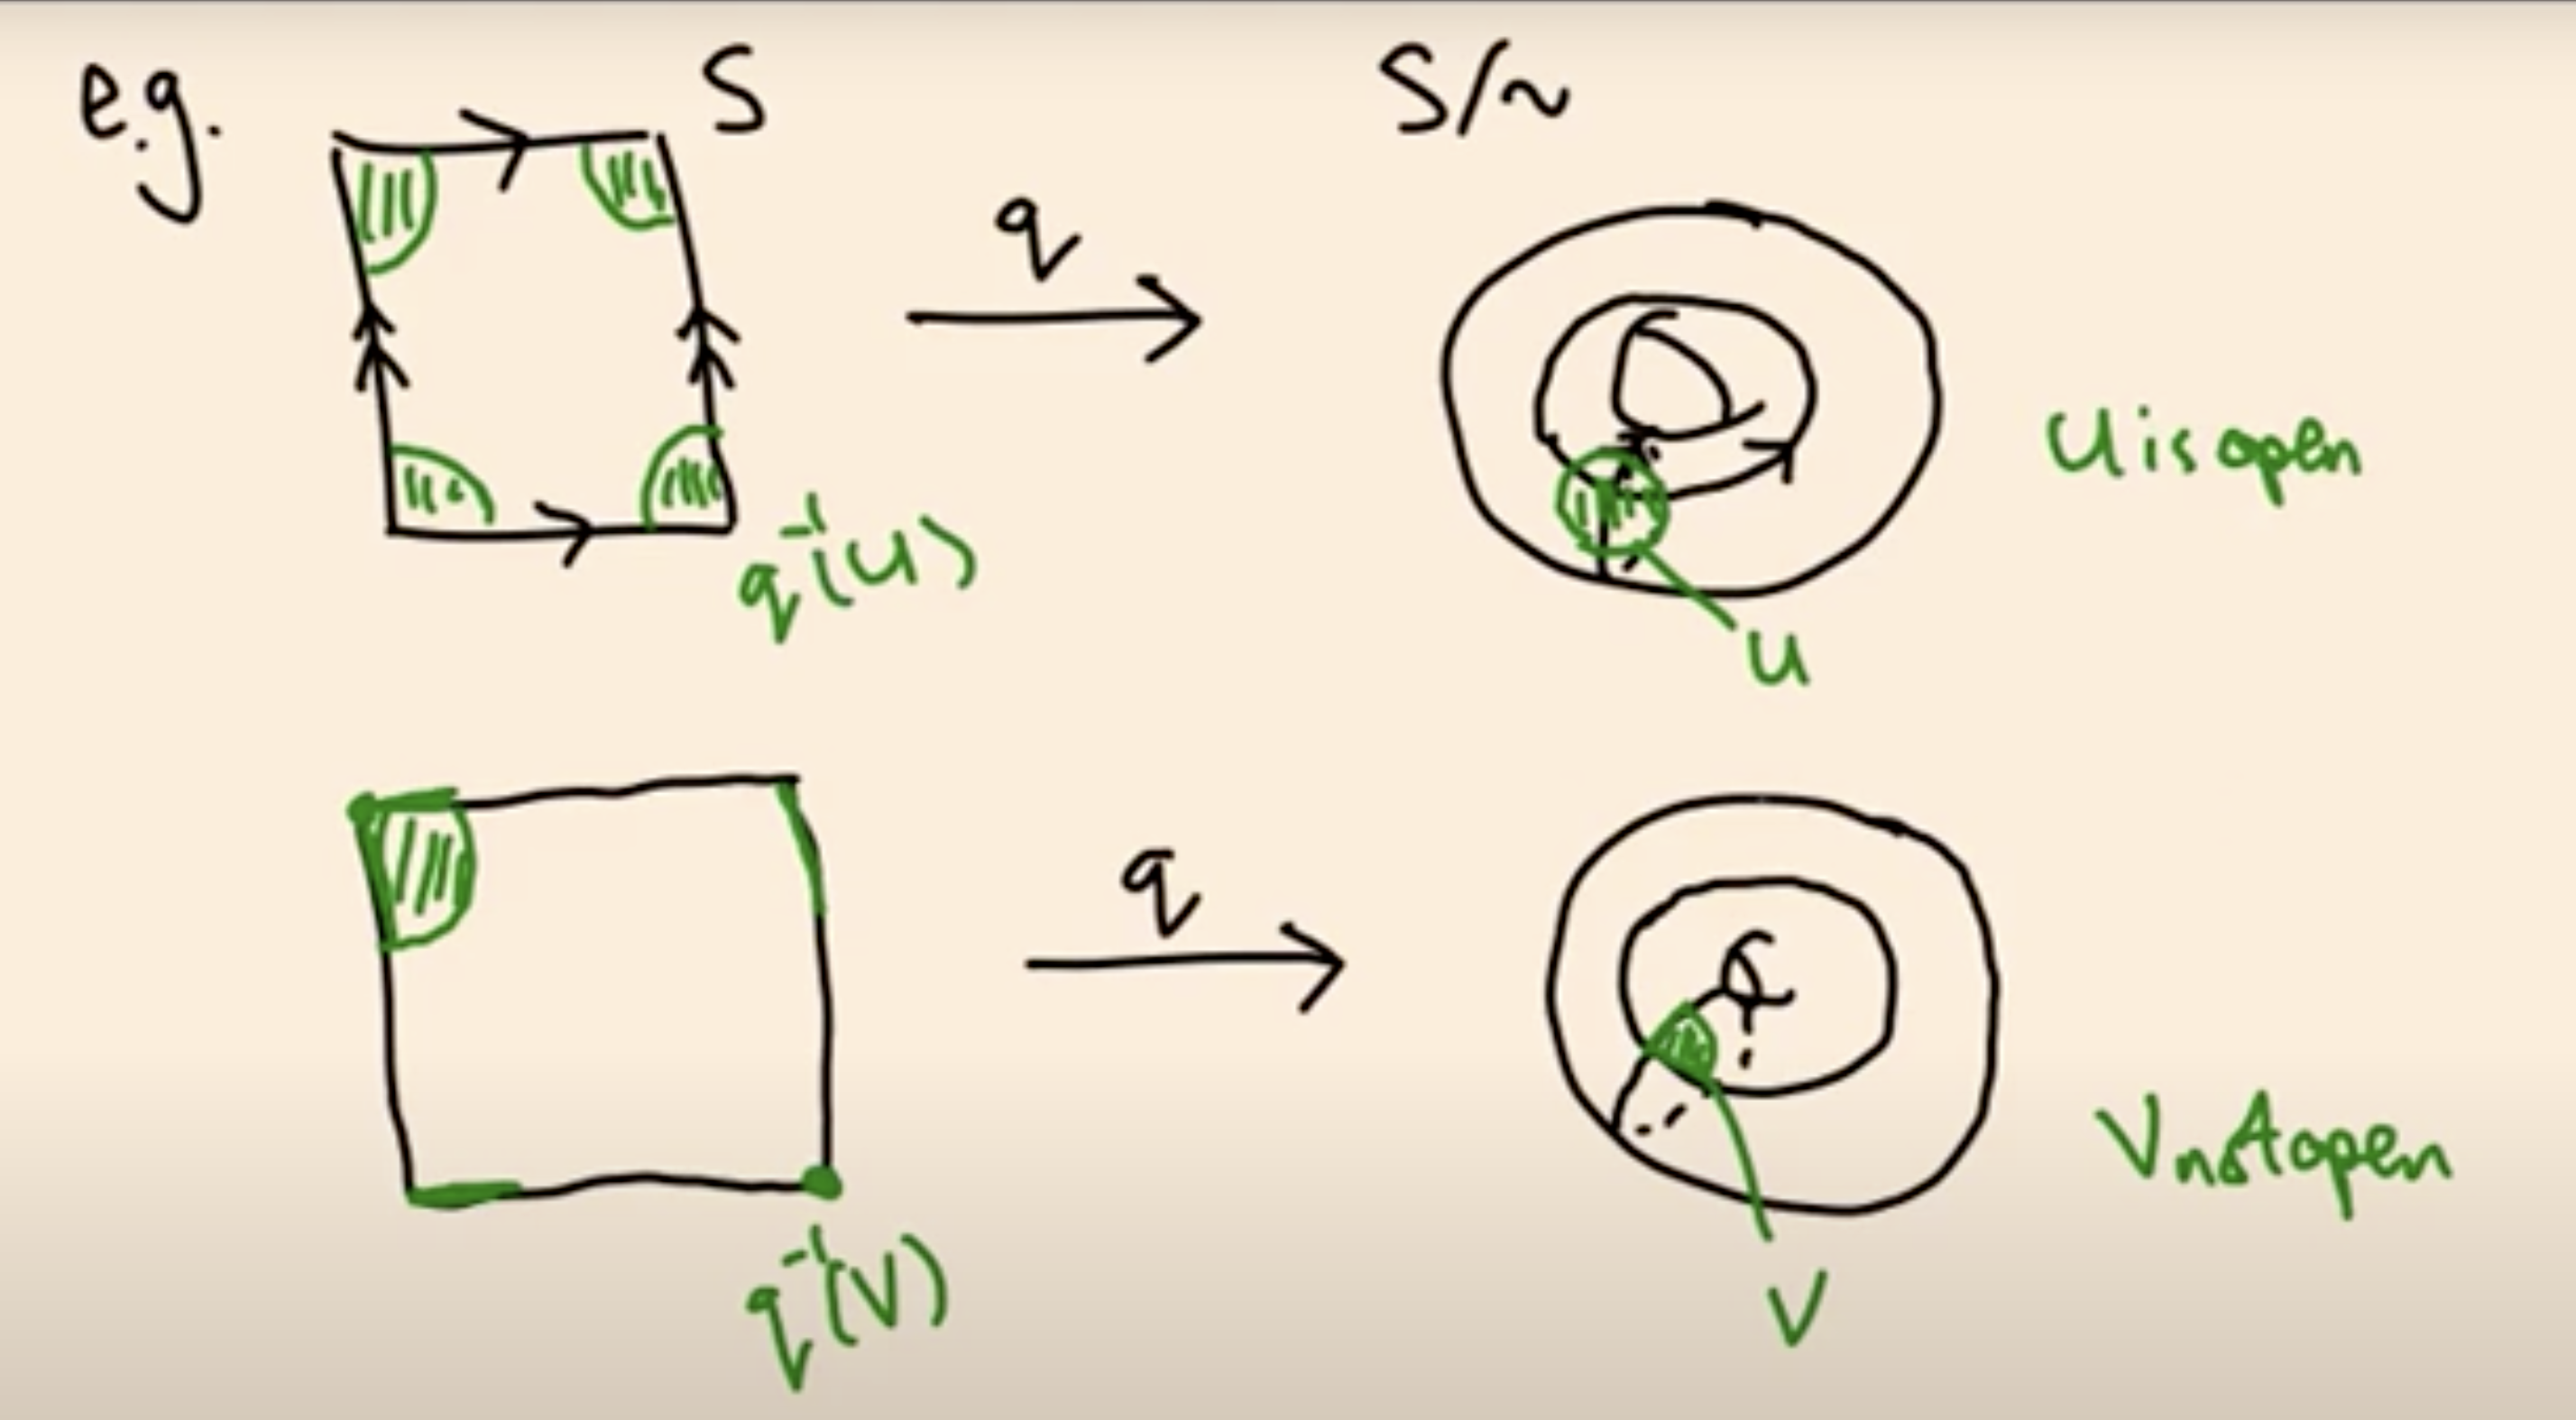
\includegraphics[width=400pt]{img/analysis--berkeley-202a-topology-f3b4.png}
    \url{https://youtu.be/aO9l7zteKlE}
  \end{mdframed}
\end{example}

The following is the key property of the quotient construction:

\begin{example}
  Let $f: X \to Y$ be a continuous map that respects the equivalence relation,
  i.e. $f(x_1) = f(x_2)$ whenever $x_1 \sim x_2$. Then there is a unique continuous map $F$ such
  that
  \begin{tikzcd}
    {X} & {X/{\sim}} \\
    & {Y}
    \arrow["{F}", from=1-2, to=2-2, dashed]
    \arrow["{q}", from=1-1, to=1-2]
    \arrow["{f}"', from=1-1, to=2-2]
  \end{tikzcd}
  commutes.
\end{example}

This says that ``the quotient is the thing that all maps agreeing on equivalence classes factor through​''.

So this seems to be saying that a continuous map on the rectangle that respects $\sim$ corresponds
uniquely to a continuous map on the torus.

\red{TODO} (me) why is $F$ continuous?

\begin{remark}
  Suppose we have a set of pairs that happen to be sent to the same thing by $f$:
  \begin{align*}
    R = \{(x, y) ~:~ f(x) = f(y) \} \subseteq X \times X.
  \end{align*}
  This is an equivalence relation. Therefore the equivalence relation generated by $R$ is contained
  in $R$ (is it not equal to $R$?)
\end{remark}

\begin{remark}
  The product is really the topological space together with the projection maps.

  The disjoint union is really the topological space together with the inclusion maps.

  The quotient is really the topological space together with the quotient map.
\end{remark}

The pushout allows us to generate many examples of topological spaces.

\begin{definition}[Pushout]
  Let $f: X \to Y$ and $g: X \to Z$ be continuous maps. The \defn{pushout} is the topological space
  \begin{align*}
    Y \pushout_X Z := \big(Y \disjunion Z\big) / {\sim}
  \end{align*}
  where $\sim$ is the smallest equivalence relation containing the pairs $f(x) \sim g(x)$ for all $x \in X$,
  together with the maps
  \begin{align*}
    \iota_Y &: Y \longrightarrow Y \disjunion Z \longrightarrow \big(Y \disjunion Z\big) / {\sim} \\
    \iota_Z &: Z \longrightarrow Y \disjunion Z \longrightarrow \big(Y \disjunion Z\big) / {\sim}.
  \end{align*}
  What does ``the smallest equivalence relation containing the pairs $f(x) \sim g(x)$​'' mean?

  We have $f(x) \in Y$ and $g(x) \in Z$; think of them as elements of $Y \disjunion Z$. We take the smallest
  equivalence relation on $Y \disjunion Z$ which contains all pairs $\(f(x), g(x)\)$. So these are pairs in the
  disjoint union of the two codomains which are united by the fact that they derive from the same $x$ in the
  shared domain. We then mod out the disjoint union by this equivalence relation. This yields equivalence
  classes in the disjoint union containing all things in $Y$ or $Z$ which come from the same $x \in X$.

  The inclusion maps $\iota_Y$ and $\iota_Z$ send an element of one of the codomains to the equivalence class
  corresponding to which $x$ is came from.
\end{definition}


This is what the quotient does: ``The quotient is the thing that all maps agreeing on equivalence
classes factor through​''.

What does the pushout do?

\begin{lemma}
  Let $u: Y \to W$ and $v: Z \to W$ be continuous maps such that
  \[
    \begin{tikzcd}
      {X} & {Y} \\
      {Z} & {W}
      \arrow["{f}", from=1-1, to=1-2]
      \arrow["{g}"', from=1-1, to=2-1]
      \arrow["{v}"', from=2-1, to=2-2]
      \arrow["{u}", from=1-2, to=2-2]
    \end{tikzcd}
  \]
  commutes. Then there is a continuous map $t: (Y \pushout_X Z) \to W$ such
  that $t \circ \iota_Y = u$ and $t \circ \iota_Z = v$, i.e.
  \[
    \begin{tikzcd}
      {X} && {Y} \\
      \\
      {Z} && {Y \pushout_X Z} \\
      &&& {} \\
      &&&& {W}
      \arrow["{f}"', from=1-1, to=1-3]
      \arrow["{g}", from=1-1, to=3-1]
      \arrow["{\iota_Z}", from=3-1, to=3-3]
      \arrow["{\iota_Y}"', from=1-3, to=3-3]
      \arrow["{t}"', from=3-3, to=5-5]
      \arrow["{u}"', from=1-3, to=5-5, curve={height=-24pt}]
      \arrow["{v}"', from=3-1, to=5-5, curve={height=18pt}]
    \end{tikzcd}
  \]
  commutes.
\end{lemma}

\begin{proof}
  We must define $t$ given $f$ and $g$. We have no choice but to set
  \begin{align*}
    t([y]) = (t \circ \iota_Y)(y) = u(y) ~~\text{for all~} y \in Y\\
    t([z]) = (t \circ \iota_Z)(z) = u(z) ~~\text{for all~} z \in Z,
  \end{align*}
  so that proves uniqueness.

  We must check it's continuous and well-defined. (well-defined follows from commutativity of
  diagram.)

  Rather than check this directly, observe that $u$, $v$ induce a continuous
  map $Y \disjunion Z \to W$. This is because a continuous map out of a disjoint union of a pair of
  sets is the same as a pair of continuous maps (``The topology of a disjoint union is set up
  precisely so that this works.​'') We will call this continuous map
  \begin{align*}
    \<u, v\>: Y \sqcup Z \to W.
  \end{align*}
  It sends an element $y$ of the disjoint union (i.e. an element that was contributed by $Y$)
  to $u(y)$, and an element $z$ of the disjoint union (i.e. an element that was contributed by $Z$)
  to $v(z)$.

  Observe that applying $\<u, v\>$ to an element $f(x)$ of the disjoint union yields
  \begin{align*}
    \<u, v\>(f(x))
    &= u(f(x)) \\
    &= v(g(x)) ~~~~~~~\text{\small by commutativity of the diagram given in the hypothesis} \\
    &= \<u, v\>(g(x)).
  \end{align*}
  So we have a continuous map that sends the generating pairs of the equivalence relation to the
  same element of $W$, i.e. if $q_1 \sim q_2$ then $\<u,v\>(q_1) = \<u,v\>(q_2)$. Thus we get a
  continuous map
  \begin{align*}
    t = \bar{\<u,v\>}:(Y \disjunion Z)/{\sim} \longrightarrow W
  \end{align*}
  with the desired property.
\end{proof}



\begin{example}
  \begin{definition}
    The $n$-sphere is
    \begin{align*}
      S^n := \{x \in \R^{n+1} ~:~ \norm{x} = 1\} \subset \R^{n+1}.
    \end{align*}
    I.e. it is the $n$-dimensional surface of an $(n+1)$-dimensional disc. For example $S^1$ is the
    unit circle in $R^2$ and $S^0 = \{-1, 1\}$.

    The $n$-disc is
    \begin{align*}
      D^n := \{x \in \R^{n} ~:~ \norm{x} \leq 1\} \subset \R^{n}.
    \end{align*}
    There is a continuous map $\iota: S^{n-1} \to D^n$, via inclusion, e.g.
    \begin{align*}
      S^0 \hookrightarrow D^1 = [-1, 1]
    \end{align*}
    e.g. $-1 \in S^0 \mapsto -1 \in [-1, 1]$
  \end{definition}


  ``This is the simplest case of constructing a C-W complex​''.

\begin{mdframed}
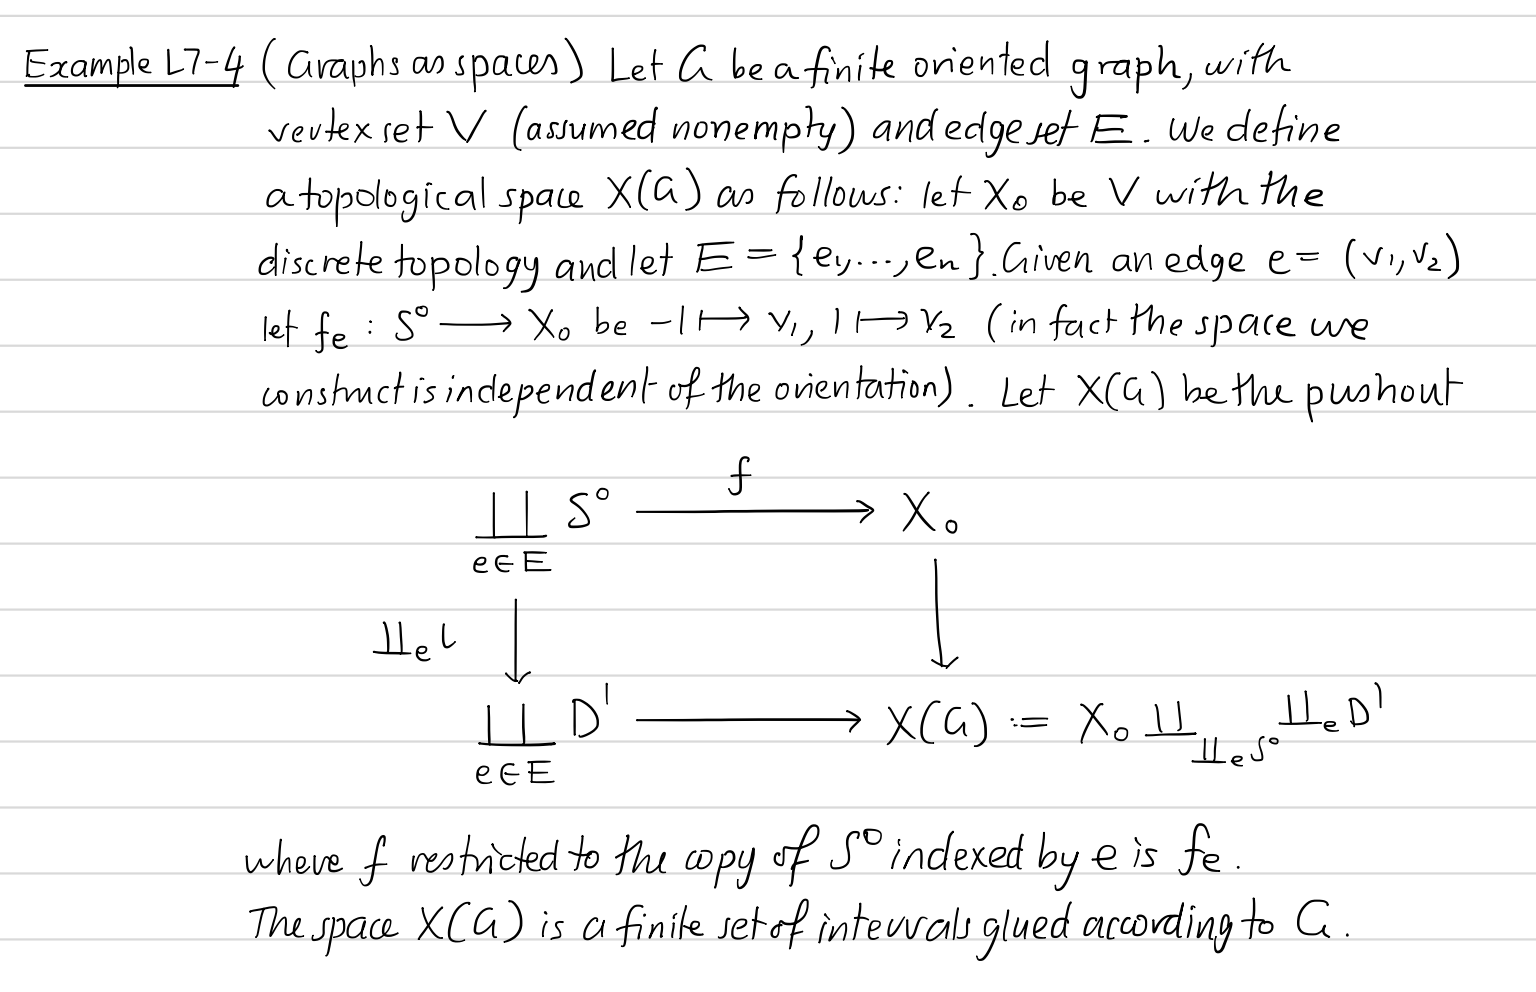
\includegraphics[width=400pt]{img/analysis--berkeley-202a-topology-0021.png}
\end{mdframed}
So: $S^0$ is being used to represent a pair of vertices. $D^1$ is being used to represent an edge.

We start off with $\disjunion_{e \in E} S^0$. This is a set of pairs of vertices; one pair for each
edge.

$f$ maps this to a set of vertices, whereas $\disjunion_e \iota$ maps it to a set of edges.

The pushout collects all these edges and vertices together, and identifies those that derive from
the same edge.

$f_e: S^0 \to X_0$ defined by $-1 \mapsto v_1$ and $1 \mapsto v_2$ is continuous ( ``$S^0$ is a pair
of points with the subspace topology in $\R^1$​, so it's discrete. Any map out of a discrete space
is a continuous map, because every subset is open. So to specify a continuous map $S^0 \to X_0$ we
just need to specify a pair of points of $X_0$.'') $f$ is the map out of the disjoint union
comprising one copy of $S^0$ for each edge $e$; the restriction of $f$ to the copy of $S^0$
corresponding to $e$ is $f_e$. This makes $f$ a continuous map also (because preimage of a union is
union of preimages and thus open I think).

$\disjunion_e \iota$ sits each pair of points at the endpoints of an interval. It is also
continuous, for similar reason to $f$ since it involves a disjoint union.

So basically, $f$ is sitting vertices in a discrete topological space, whereas $\disjunion_e \iota$
is sitting vertices at the endpoints of edges. The topological space associated to the graph $G$ is
the pushout of these two continuous maps. It takes the disjoint union of (the set of all vertices)
and (a set of lines, one per edge) and glues them together such that the diagram commutes.

\begin{mdframed}
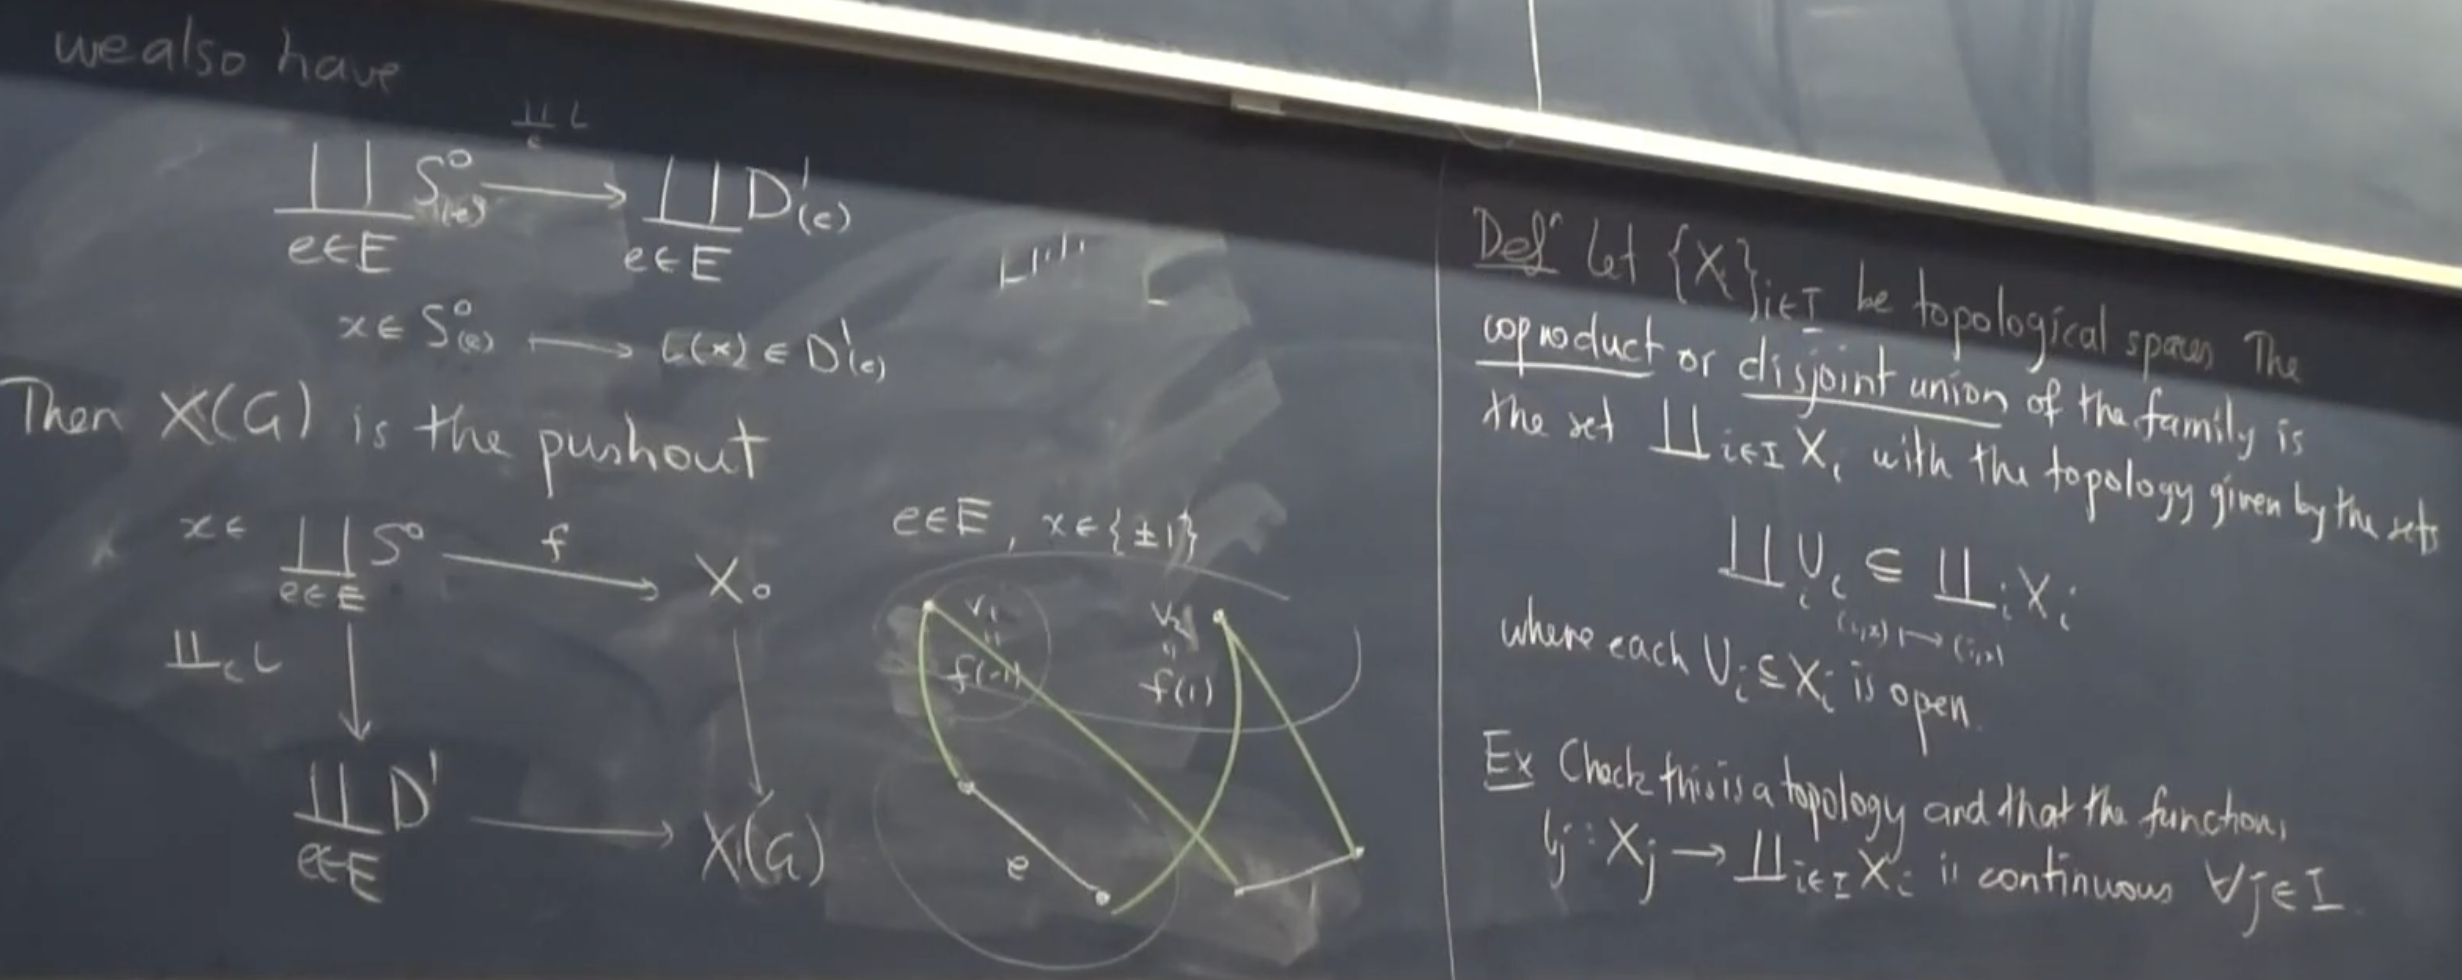
\includegraphics[width=400pt]{img/analysis--berkeley-202a-topology-54da.png}
\end{mdframed}
\end{example}


\begin{definition}[homeomorphism]
  A continuous map $f:X \to Y$ is a \defn{homeomorphism} if it is a bijection with continuous inverse.

  Equivalently, if there exists a continuous map $g:Y \to X$ with $g \circ f = 1_X$ and $f \circ g = 1_Y$.

  We write $X \cong Y$.
\end{definition}

\begin{remark}
  With groups the following is true:

  {\it A homomorphism is an isomorphism iff it is a bijection.}

  This is not true for homeomorphism: the inverse must be continuous ($f$ must send open sets to open sets)
\end{remark}

\begin{example}[circle as quotient]
  Let $X = [0, 1]/{\sim}$ where $\sim$ is generated by the pair $0 \sim 1$.

  (I.e. there's an equivalence relation in which $0$ and $1$ are identified with each other in an equivalence
  class with two elements, and every other point is in an equivalence class of its own.)

  \begin{lemma}
     $X \cong S^1$, a circle.
  \end{lemma}

  \begin{proof}
    We must exhibit a homeomorphism between the topological spaces $X = [0, 1]/{\sim}$ and $S^1$.

    Recall that the continuous maps out of a quotient space $[0, 1]/{\sim}$ are in bijection with the
    continuous maps out of $[0, 1]$ which respect $\sim$ (the universal property of the quotient) i.e.
    \begin{align*}
      \cts([0, 1]/{\sim}, Y) \cong \Big\{f: [0, 1] \to Y ~:~ f(0) = f(1)\Big\}.
    \end{align*}
    Thus a homeomorphism is
    \begin{align*}
      [x] &\mapsto (\cos 2\pi x, \sin 2 \pi x) \\
      [x] &\mapsto (1, 2\pi x) ~~~~~\text{\small in polar coordinates}
    \end{align*}
  \end{proof}

  \begin{quote}
    So $[0, 1]/{\sim}$ is an interval where we gave declared the endpoints to be the same point.
    And $S^1$ is a circle in $\R^2$. And these are the {\it same topological space}. But we don't need to think
    of $[0, 1]/{\sim}$ as being embedded in $\R^2$, i.e. we don't have to imagine ``bending it
    around​'' to make the endpoints meet. It's just that they are the same topological space; i.e.
    there is a bijection between their points and each point has the same set of neighborhoods.
  \end{quote}
\end{example}

\begin{example}[circle as pushout]
  Here, $\{*\}$ is the one-point topological space.
  \[
    \begin{tikzcd}
      {\{*\} \disjunion \{*\}} && {\{*\}} \\
      \\
      {[0, 1]} && {(\{*\} \disjunion [0,1])/{\sim}}
      \arrow[from=1-1, to=1-3]
      \arrow["f"', from=1-1, to=3-1]
      \arrow[from=3-1, to=3-3]
      \arrow[from=1-3, to=3-3]
    \end{tikzcd}
  \]
  The disjoint union $\{*\} \disjunion \{*\}$ is $\{*_1, *_2\}$, say. $f$ is a map that
  sends $*_1 \mapsto 0$ and $*_2 \mapsto 1$.

  The above construction represents the following:

  We have two separate topological spaces: the interval $[0, 1]$ and a single point.

  Following the diagram starting with $*_1$ yields an equivalence class containing $*$ and $0$;
  following the diagram starting with $*_2$ yields an equivalence class containing $*$ and $1$.

  So we have identified a single point with the two endpoints of the interval, and in so doing have
  created something homeomorphic to the circle $S^1$ again:
  \begin{align*}
    \(\{*\} \disjunion [0,1]\)/{\sim} \cong [0,1]/{\sim} \cong S^1.
  \end{align*}
\end{example}

\begin{quote}
  Suppose $f$ and $g$ are injective. Then the spaces $Y$ and $Z$ share a common subspace
  (corresponding to a copy of $X$), and the pushout is gluing $Y$ and $Z$ together along that
  common piece.
\end{quote}
\begin{mdframed}
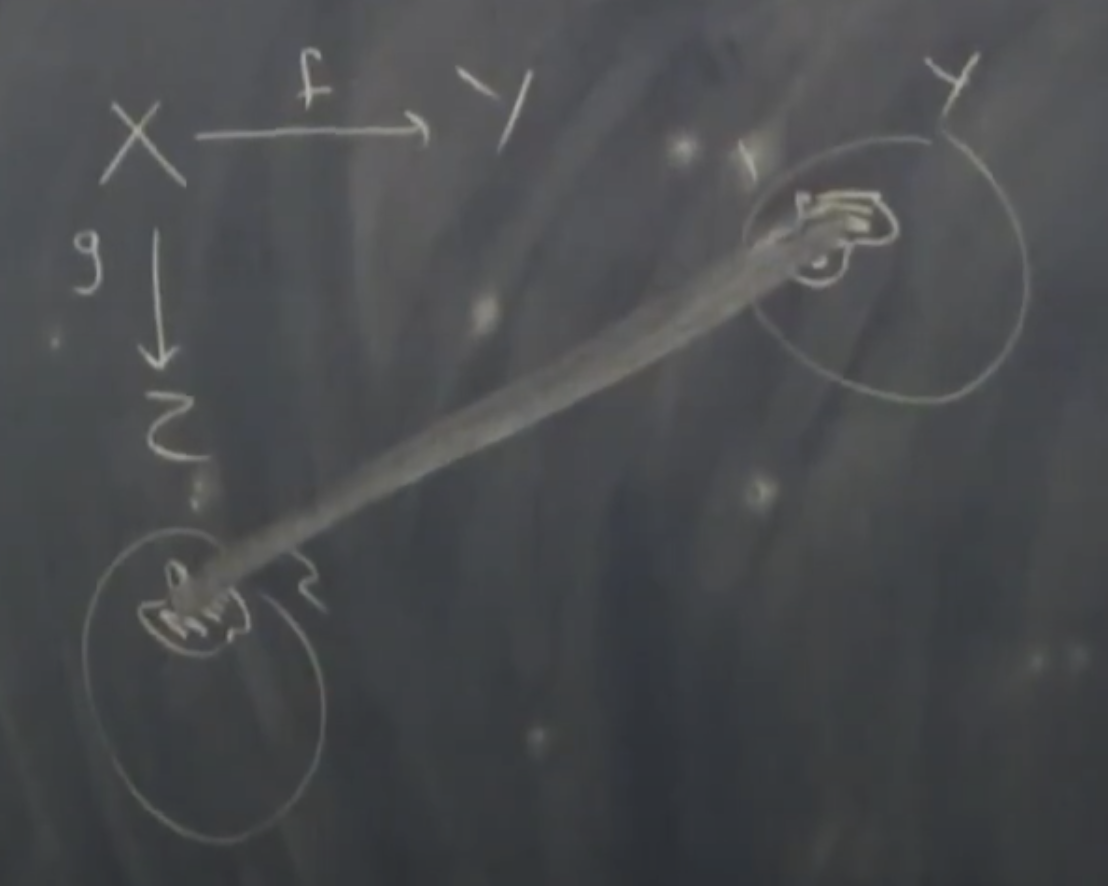
\includegraphics[width=400pt]{img/analysis--berkeley-202a-topology-0f64.png}
\end{mdframed}

\begin{example}
  Let $Y$ be the surface of a ``pair of pants​'' in $R^3$, and let $Z$ be a ``cylinder that bifurcates
  and the rejoins​'' (two copies of $Y$ in opposite orientations, glued at their foot holes). $f$
  and $g$ are maps that include the circle in $Y$ and $Z$ respectively (i.e. $f$ maps the
  circle $S^1$ to the circle which is embedded in $Y$ which forms the ``opening​'' of $Y$ at the waist
  end. And $g$ does the same for one of the openings of $Z$.) The pushout defines a gluing of $Y$
  and $Z$:
\begin{mdframed}
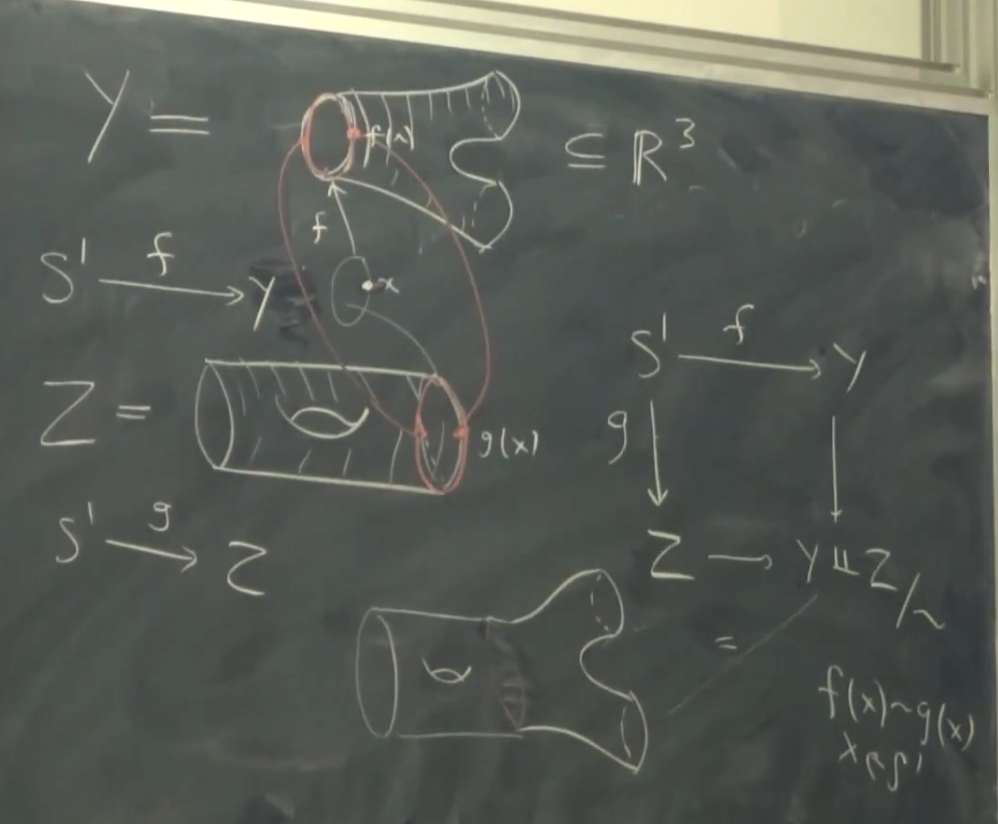
\includegraphics[width=400pt]{img/analysis--berkeley-202a-topology-889a.png}
\end{mdframed}
\end{example}

\begin{example}[Torus, Mobius strip]
\begin{mdframed}
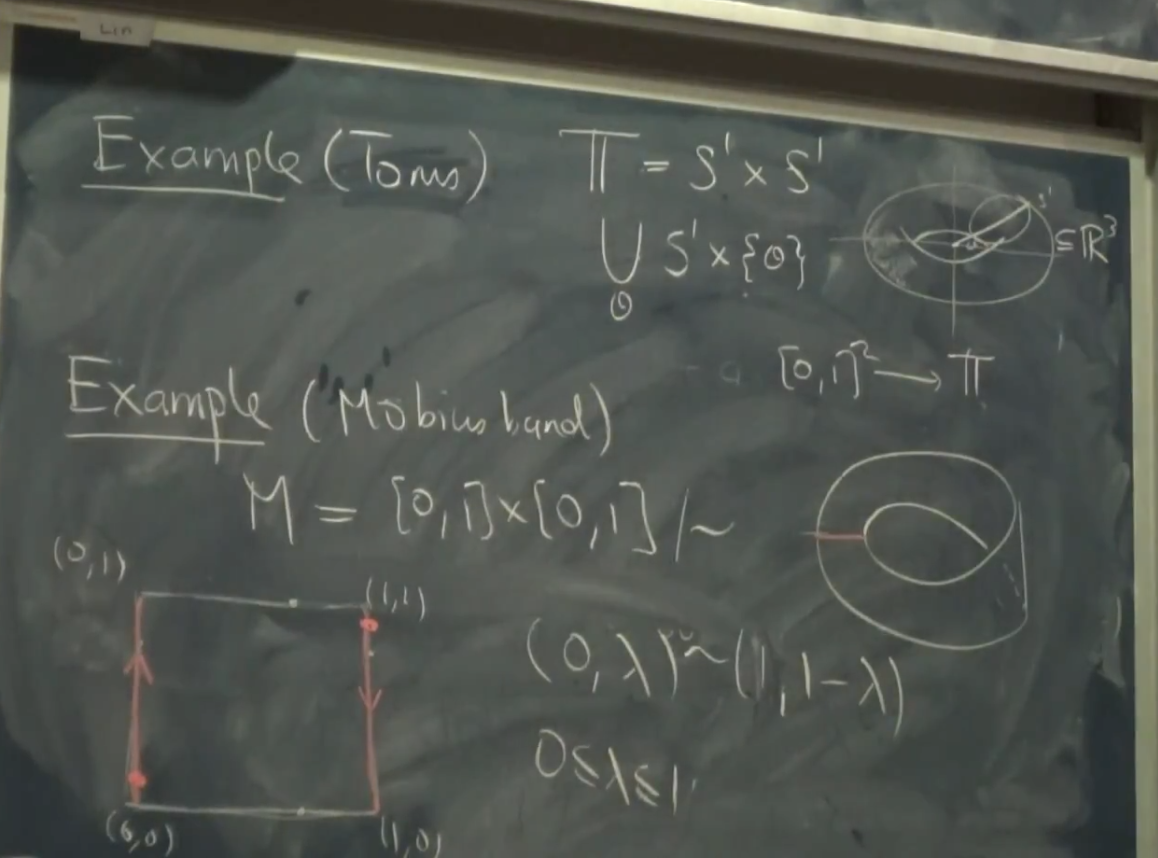
\includegraphics[width=400pt]{img/analysis--berkeley-202a-topology-9b96.png}
\end{mdframed}
\end{example}


\begin{question}
  How do we determine whether $X \cong Y$? (Usually you have them in the form of algorithms for constructing
  them.) This is a hard question.

  For example, $M \not\cong S^1 \times [0, 1]$. It would be true if we just formed a strip of paper
  into a ring and glued one edge. But the gluing for the Mobius strip involved twisting, so we
  expect these not to be homeomorphic.

  Also $\mathds{T} \not\cong S^2$ the torus is not homeomorphic to the 2-sphere.

  Also $S \not\cong \R$ (the former is compact, the latter isn't).

  Also $\R^n \not\cong \R^m$ when $n \neq m$, but this is only obvious for $n=1, m=2$.

  Telling topological spaces apart often involves computing invariants (e.g. a number, or vector
  space, associated with a topological space) and comparing them. For example, the ``first homology
  group of the torus is two-dimensional​'' which means that there are only two different ``sort​'' of
  circles that exist inside a torus: one sort going around the hole and another not; the homology
  group is spaned by these two sorts of circles.
\end{question}

Recall $S^{n-1} \xhookrightarrow{\rm \iota} D^n$ (an $n$-disc or $n$-cell).

\begin{definition}
  A topological space $Y$ is obtained from $X$ by \defn{attaching n-cells} if there exists a family of continuous
  maps
  \begin{align*}
    \{f_\alpha ~:~ S^{n-1} \to X\}_{\alpha \in \Lambda}.
  \end{align*}
  (called attaching maps) and a pushout

\begin{mdframed}
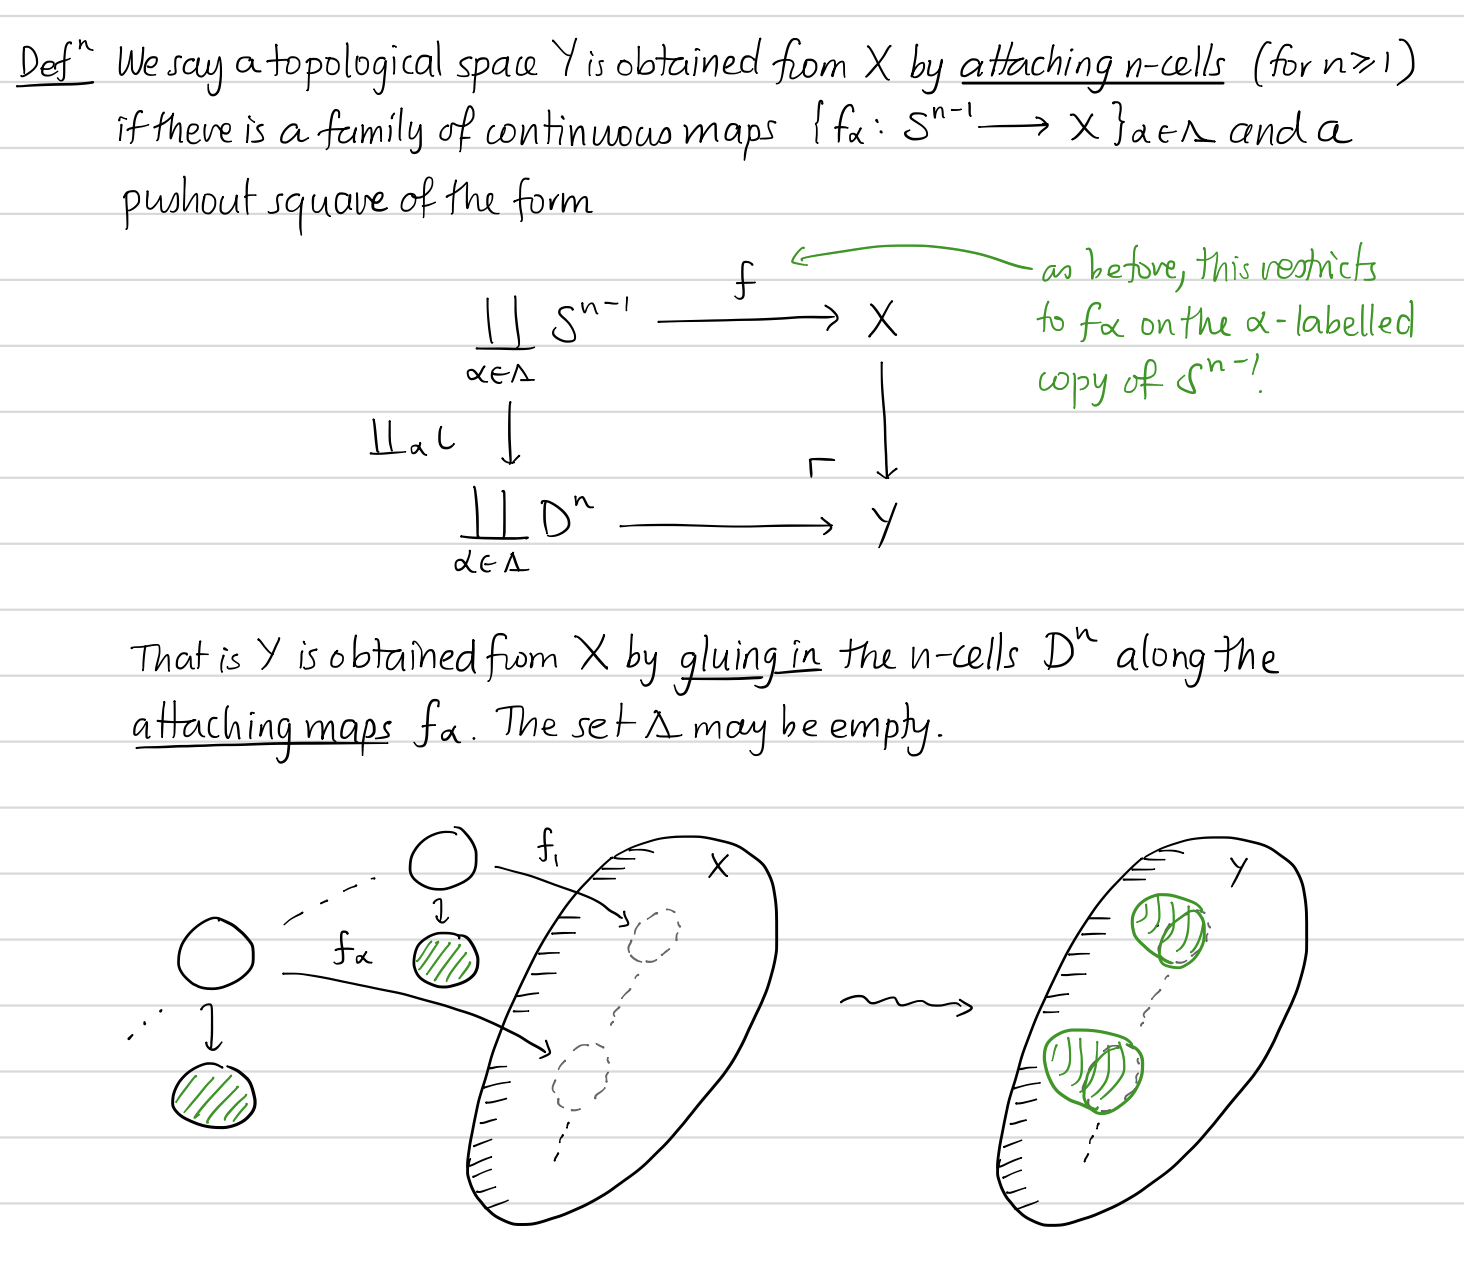
\includegraphics[width=400pt]{img/analysis--berkeley-202a-topology-55c5.png}
\end{mdframed}
\end{definition}

\begin{definition}
  \begin{mdframed}
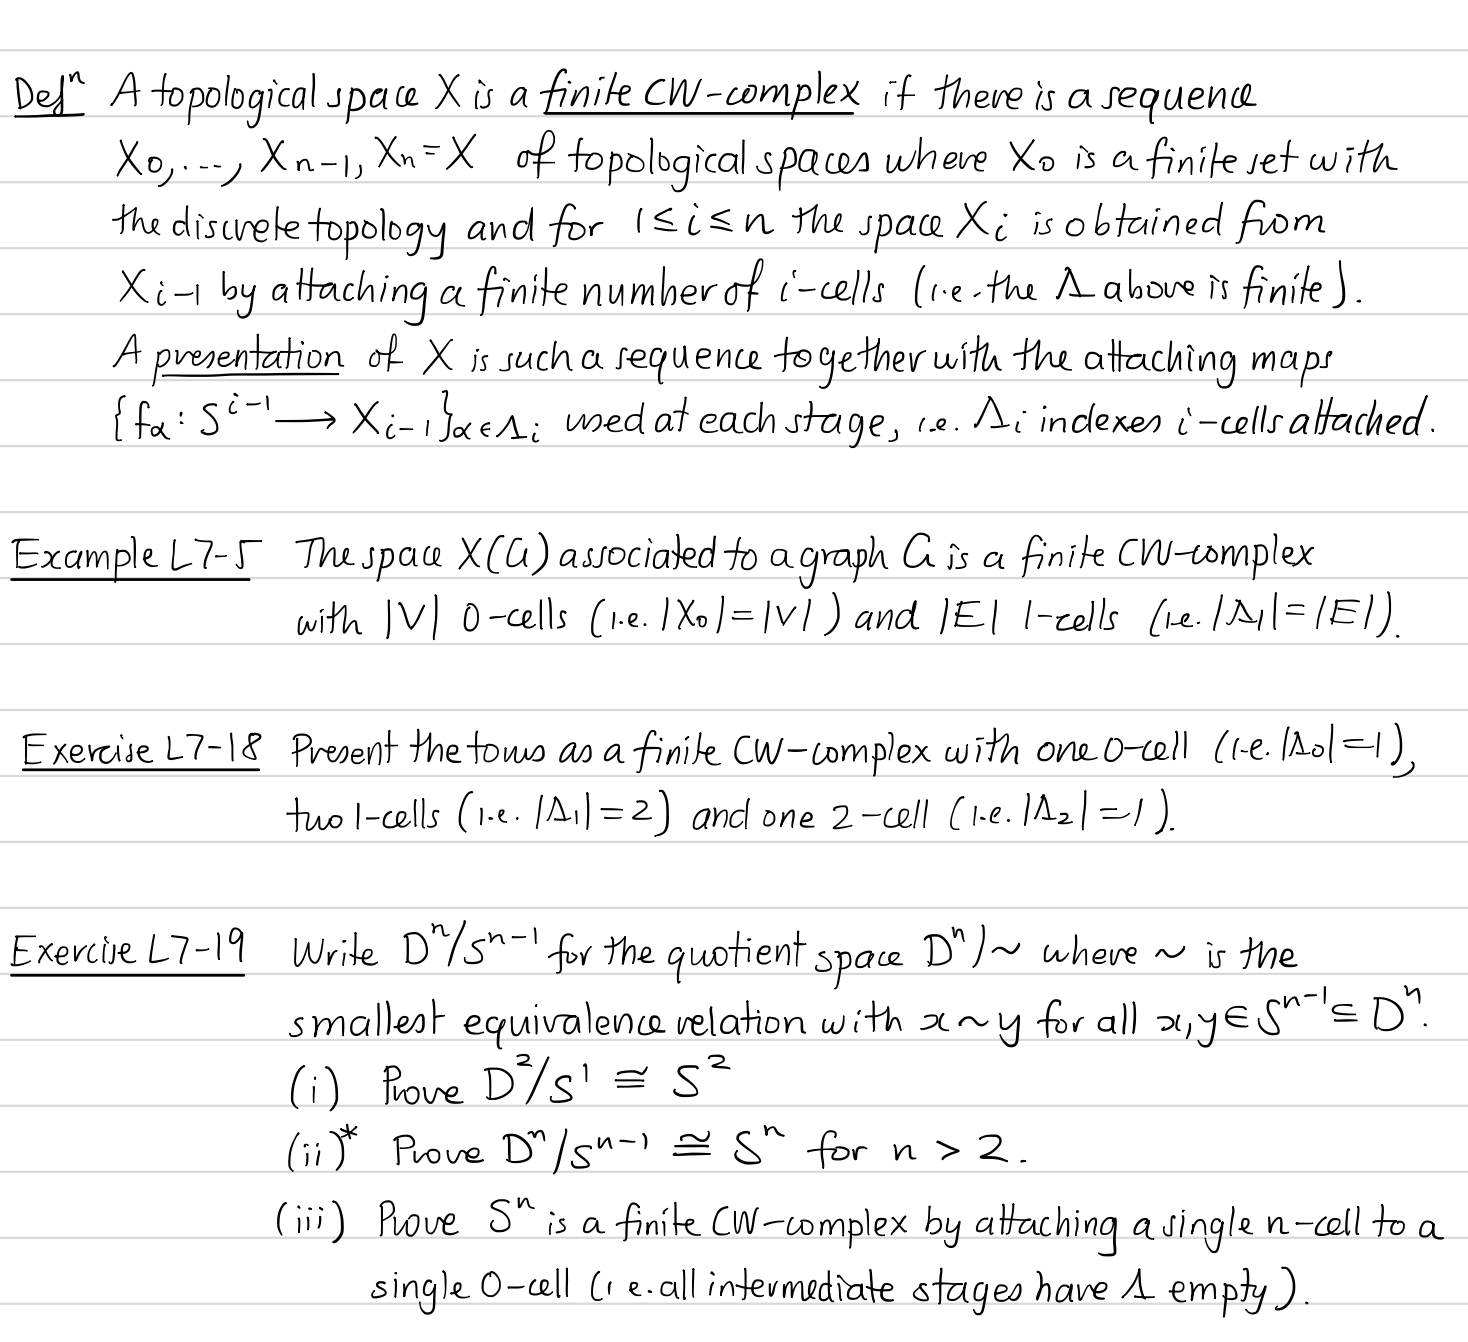
\includegraphics[width=400pt]{img/analysis--berkeley-202a-topology-ec33.png}
\end{mdframed}
\end{definition}

\section{Compact spaces}

$[a, b]$ is compact; $\R$ is not. In some sense it has to do with finiteness. Although we will
define it in a metric space setting first, it is actually a topological property, although it's
topological definition is less intuitive.

We know three things about intervals:
\begin{enumerate}
\item Extreme value theorem: a continuous map on an interval is bounded and it attains its extrema.
\item A continuous function on an interval is uniformly continuous.
\item The Riemann integral exists for a continuous function on an interval.
\end{enumerate}

These are all explained by compactness.

We will define compactness for arbitrary metric spaces. Then the first two will work for any
compact metric space. Then the notion of compactness, or functions with compact support, will be
the point we start from to talk about Riemann integrals over compact subsets of $\R^n$, and thence
to Lebesgue integrals without measure theory. Then the part of the course about Hilbert spaces will
revolve around Lebesgue integrals.

\begin{definition}
  A subset $X \subseteq \R$ is \defn{bounded} is there exists $M$ such that $X \subseteq [-M, M]$ (or $(-M, M)$,
  doesn't matter).

  A point $x \in \R$ is an \defn{adherent point} of $X$ is either of the following equivalent conditions are true:
  \begin{enumerate}
  \item there exists a sequence $(a_n)_{n=0}^\infty$ in $X$ converging to $x$
  \item $\forall \eps > 0 ~ \exists y \in X(|x - y| < \eps)$ (I think that's equivalent to: every neighborhood
    of $x$ contains a point of $X$)
  \end{enumerate}
  $X$ is \defn{closed} if it contains all its adherent points.
\end{definition}

\begin{lemma}
  $X \subseteq \R$ is closed in this sense iff it is closed in the topology on $\R$.
\end{lemma}

\begin{proof}
  $\implies$\\
  We must show that $X^c \in \mc T_X$, where $\mc T_X$ is the topology induced by the standard metric on $\R$.

  Let $x \in X^c = \R \setminus X$. Then its not an adherent point of $X$ so we can place a open
  ball around it without leaving $X^c$, hence $X^c$ is open.

  $\impliedby$\\
  $X^c$ is open so for every $x \in X^c$ we can place an open ball around it without capturing a point of $X$,
  so $x$ is not an adherent point of $X$, so $X$ contains its adherent points.
\end{proof}

\begin{theorem}[Bolzano-Weierstrass]
  A subset $K \subseteq \R$ is closed and bounded if and only if every sequence in $K$ has a
  subsequence that converges to a point in $K$.
\end{theorem}

\begin{intuition}
  (Me) Suppose a sequence in $K$ lacked a subsequence converging to a point in $K$. Then everywhere
  you look in $K$, you'd be able to take $\eps$ sufficiently small that an open ball will not
  capture any points of the sequence (except possibly at its centre). I think B-W is saying that a
  subset is closed and bounded iff it doesn't have the ``room​'' that would be needed for that.
\end{intuition}

\begin{proof}
  $\implies$\\
  (Me) $K$ is closed (contains its adherent points) and bounded. Let $M$ be the bound. When the
  sequence lays down its $n$-th point, consider the maximum distance that point can be from the
  closest previous point. That distance is always decreasing. ... this probably isn't fruitful.

  $\impliedby$\\
  We have that every sequence has a subsequence that converges in $K$.

  Suppose it is not closed. Then we could take a sequence that converges to a point $x$ outside $K$
  (e.g. $y_n = B(x, 2^{-n}) \cap K$). By hypothesis there is a subsequence converging to $y \in K$.
  But limits are unique (can't have a subsequence converging to a different value), hence $x = y$.
  Contradiction.

  (Me) Suppose it is not bounded: then we could take a sequence like $1, 2, \ldots$ and that would
  not have a convergent subsequence. Contradiction.
\end{proof}

\begin{lemma}
  If a sequence in a metric space has a limit then it is unique.
\end{lemma}

\begin{lemma}
  $\limninf f(x_n) = f(\limninf x_n)$ for continuous f.
\end{lemma}

\begin{definition}
  A metric space $(X, d)$ is \defn{sequentially compact} if every sequence in $X$ contains a convergent
  subsequence.
\end{definition}

I.e. the analog of closed and bounded in $\R$.

\begin{lemma}
  Let $(X, d)$ be a sequentially compact metric space and $f: (X, d_X) \to (Y, d_Y)$ is a
  continuous map. Then the image $f(X)$ is sequentially compact.
\end{lemma}



\begin{definition*}
  A topology on $X$ is \defn{metrizable} if there exists a metric on $X$ that induces it.
\end{definition*}


\begin{theorem}
  For a metric space $X$,
  \begin{align*}
    \text{second countable} \iff \text{separable}.
  \end{align*}
\end{theorem}

\begin{definition}
  directed set

  net

  converges
\end{definition}


\begin{theorem}[Bass 20.8 nets, convergence, limit points]
  \red{TODO}
\end{theorem}

Murfet
\begin{quote}
  The point of a topology is to pick out which functions are continuous.
\end{quote}

\begin{definition}
  $f: (X, \mc T) \to (Y, \mc U)$ is \defn{continuous} if the preimage of every open set is an open set.

  open function

  homeomorphism
\end{definition}

\begin{example}[cts]
  $\text{cts}(X, Y)$ is the set of continuous functions.

  Consider $\cts(\{*\}, X)$, the set of continuous functions from a singleton set to a topological space $X$.

  A singleton set has a unique topology: the ``one point​'' topology: $\{\emptyset, X\} = \{\emptyset, \{*\}\}$.

  What is the set $\cts(\{*\}, X)$, i.e. the continuous maps from a singleton to an arbitrary topological
  space?

  Every map is of the form $* \mapsto x$ for some $x \in X$. So the preimage is open ($\{*\}$) for every map
  and therefore every map on the singleton set is continuous (it's the discrete topology, as well as the
  indiscrete topology) and they are in bijection with $X$: $\cts(\{*\}, X) \cong X$. (Each map corresponds to a
  choice of some $x$)
\end{example}

\begin{example}[Sierpinski space]
  $\Sigma = \{0, 1\}$.
  $\mc T = \{\emptyset, \Sigma, \{1\}\}$
  Claim: not metrizable.

  What does $\cts(X, \Sigma)$ look like for an arbitrary topological space $X$?

  Let $f \in \cts(X, \Sigma)$. Each $f$ is a characteristic function of some open subset of $X$.

  We can write
  \begin{align*}
    \cts(X, \Sigma) \hookrightarrow \powerset(X)
  \end{align*}
  meaning (I think) that there exists an injective map from the set of continuous maps to the
  powerset. This is because each continuous map corresponds to an open subset of $X$, i.e. the
  continuous maps are in bijection with a subset of the powerset. Specifically, this injective map
  could be
  \begin{align*}
    f \mapsto f^{-1}(1)
  \end{align*}
  (it could also be $f \mapsto f^{-1}(0)$).

  So we can also say there is a bijection
  \begin{align*}
    \cts(X, \Sigma) \to \mc T
  \end{align*}
  ($f$ is sent to the open set of which it is the characteristic function, and the open set is sent
  to its characteristic function).

  Remark: if $G$ is open in $X$ then the characteristic function $\ind_G$ is continuous,
  since $\{1\}$ is the only open set in the codomain in $\Sigma$ and its preimage is $G$.
\end{example}


Murfet:
\begin{quote}
  If you know all the continuous maps $X \to Y$ out of a topological space for all $Y$ then you
  know $\mc T_X$ (because you can look at the maps to the Sierpinski space, and these are indicator
  functions of open sets in $X$).

  This is the sense in which the notion of continuity is more fundamental than that of topology (i.e. the
  category theory point of view).

  The purpose of a topology $\mc T$ is to tell you which functions out of $X$ are continuous. If
  you know that, you can recover the topology.
\end{quote}

Question: But is it realistic to think that one would ``know all the continuous maps $X \to Y$ out
of a topological space​''?

\begin{lemma}
  A function between metric spaces is continuous in the metric space sense if and only if it is
  continuous in the topological sense.
\end{lemma}

\begin{proof}
  Let $f: (X, d_X) \to (Y, d_Y)$, and let $\mc T_X$ and $\mc T_Y$ be the topologies induced by the
  metrics.

  $\impliedby$\\
  Suppose $f$ is continuous in the topological sense. Given $x \in X$ and $\eps$, we must exhibit
  a $\delta$. Let $U = f^{-1}(B(f x, \eps))$. We know that $U \in \mc T_X$, therefore it is open in
  the metric sense. Also $x \in U$. Therefore we may take any $\delta$ such
  that $B(x, \delta) \subseteq U$.

  $\implies$\\
  Suppose $f$ is continuous in the metric space sense. Let $V \in \mc T_Y$. We must show
  that $f^{-1}(V) \in \mc T_X$.

  Let $x \in f^{-1}(V)$. We must exhibit $\delta$ such that $B(x, \delta) \subseteq f^{-1}(V)$.
  But $V$ is open and $f$ is continuous in the metric sense. Therefore we may take a
  ball $B(f x, \eps) \subseteq V$ and there will exist such a ball $B(x, \delta)$.
\end{proof}





\begin{theorem}
  Let $f: (X, \mc T) \to (Y, \mc U)$. If $\mc S$ is a subbase for $Y$ then $f$ is continuous
  if $f^{-1}(G) \in \mc T$ for all $G \in S$.
\end{theorem}

\begin{proof}
  \red{TODO}
\end{proof}




\section{Compactness}

\begin{definition}
  Let $(X, \mc T)$ be a topological space and let $A \subset X$.

  $\mc O \subseteq \mc T$ is an \defn{open cover} of $A$ if $A \subseteq \bigcup \mc O$.

  $\mc O$ may be uncountable.

  A \defn{subcover} is a subset of an open cover that still covers.

  $A$ is \defn{compact} if every open cover has a finite subcover.
\end{definition}

So, if there's any open cover for which it's not possible to find a finite subcover, then that's non-compact.

\begin{theorem*}[20.11]
  $A$ is compact if $A \subset B$ with $A$ closed and $B$ compact.
\end{theorem*}

\begin{proof}
  \red{TODO}
\end{proof}

\begin{theorem}[20.12]
  Image of a compact subset under a continuous map is compact.

  I.e. $f(A)$ is compact if $f: X \to Y$ is continuous with $A \subset X$ compact.
\end{theorem}

\begin{theorem*}[20.13]
  \red{TODO}
\end{theorem*}

\section{Tychonoff's theorem}

\red{TODO}

\section{Compactness and metric spaces}

\begin{definition*}
  A set $A$ is \defn{bounded} if there exists $x_0 \in A$ and $M > 0$ such that $A \subseteq B(x_0, M)$.
\end{definition*}

\begin{theorem*}
  In a metric space
  \begin{align*}
    \text{compact} \implies \text{closed and bounded}
  \end{align*}
\end{theorem*}

\begin{proof}
  \red{TODO}
\end{proof}

\begin{theorem}[20.22 Heine-Borel]
  In $\R^n$
  \begin{align*}
    \text{compact} \iff \text{closed and bounded}
  \end{align*}
\end{theorem}

\begin{proof}
  \red{TODO}
\end{proof}

\begin{definition}
  \defn{Bolzano-Weierstrass property}

  \defn{Sequentially compact}
\end{definition}

\begin{theorem}[20.21]
  The following are equivalent:
  \begin{enumerate}
  \item $A$ is compact
  \item $A$ has the Bolzano-Weierstrass property
  \item $A$ is sequentially compact
  \end{enumerate}
\end{theorem}

\begin{definition}
  \defn{complete}

  \defn{totally bounded}
\end{definition}

\begin{theorem}[20.23]
  In a metric space
  \begin{align*}
    \text{compact} \iff \text{complete and totally bounded}
  \end{align*}

\end{theorem}


\begin{theorem*}
  A continuous function from a compact metric space to a metric space is uniformly continuous.
\end{theorem*}


\begin{definition*}
  isometry of a metric space

  completion of a metric space
\end{definition*}

\begin{theorem*}
  Every metric space has a completion.
\end{theorem*}

\section*{Separation properties}

\begin{definition*}

  $X$ is a $T_1$ \defn{space} if whenever $x \neq y$ there exists $G$ with $x \in G$ and $y \notin G$.

  \defn{Hausdorff} every $x \neq y$ can be separated by {\it disjoint} open sets.

  \defn{Completely regular} A space X is a completely regular space if X is a T1 space and whenever F is a closed subset of X and x ∈/ F, there exists a continuous real-valued function f taking values in [0, 1] such that f(x)=0andf(y)=1forally∈F.

  \defn{Normal} A space X is a normal space if X is a T1 space and whenever E and F are disjoint closed sets in X, there exist disjoint open sets G and H such that E ⊂ G and F ⊂ H.

\end{definition*}

\red{TODO} propositions 20.26 - 20.30


\section{Urysohn's lemma}

\url{https://www.youtube.com/watch?v=UQas4Cu89D0}

\begin{theorem}
  If $X$ is {\it normal} and $E$ and $F$ are {\it disjoint closed} subsets, then there exists {\it continuous}
  $f: X \to [0, 1]$ such that $f$ is $0$ on $E$ and $1$ on $F$.
\end{theorem}

\begin{proof}
  \red{TODO}
\end{proof}

\begin{corollary}
  If $K \subset G \subset X$ with $X$ compact Hausdorff, $G$ open, and $K$ compact, then there exists
  continuous $f$ that is $1$ on $K$ and such that the support of $f$ is contained in $G$.
\end{corollary}

\section{Tietze extension theorem}

\begin{theorem}
  Let $F$ be closed and let $f: F \to [a, b]$ be a continuous real-valued bounded function. Then there exists a
  continuous extension $\bar f: X \to [a, b]$.

  ``Extension​'' means that $\bar f|_F = f$.
\end{theorem}

\begin{proof}
  We will define $\bar f$ as an infinite sum of functions $g_i$.
\end{proof}


\section{Connected sets}

Recall that a set is closed by definition if its complement is open.

Therefore a set is both open and closed (clopen) iff it is open and its complement is open.

Therefore (no non-trivial clopen sets) $\iff$ (cannot be partitioned into two disjoint open sets)
